\part{DC machines}
\title{DC machines}  
\date{}  
\frame{\titlepage} 

%%%%%%%%%%%%%%%%%%%%%%%%%%%%%%%%%%%%%%%%%%%%%%%%%%%%%%%%%%%%%
%% Homopolar / unipolar machines %%
%%%%%%%%%%%%%%%%%%%%%%%%%%%%%%%%%%%%%%%%%%%%%%%%%%%%%%%%%%%%%
\begin{frame}
	\frametitle{Homopolar / unipolar machines}
    \vspace{-0.3cm}
	\begin{figure}
		\centering
		\begin{subfigure}[b]{0.49\textwidth}
			\centering
			\movie{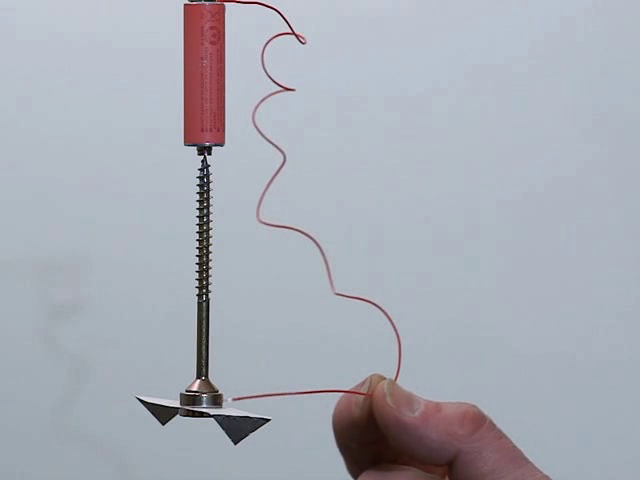
\includegraphics[height=0.4\textheight]{fig/lec03/homopolar_machine_video.png}}{fig/lec03/homopolar_machine_video.mp4}
            \vspace{0.75cm}
			\caption{Video of an operating homopolar machine (source: \href{https://de.wikipedia.org/wiki/Datei:Homopolarmotor_MAQ03891_smial_wp.ogv}{Wikimedia Commons}, Smial, \href{https://artlibre.org/licence/lal/en/}{Free Art License})}
		\end{subfigure}
		\hfill
		\begin{subfigure}[b]{0.49\textwidth}
			\centering
			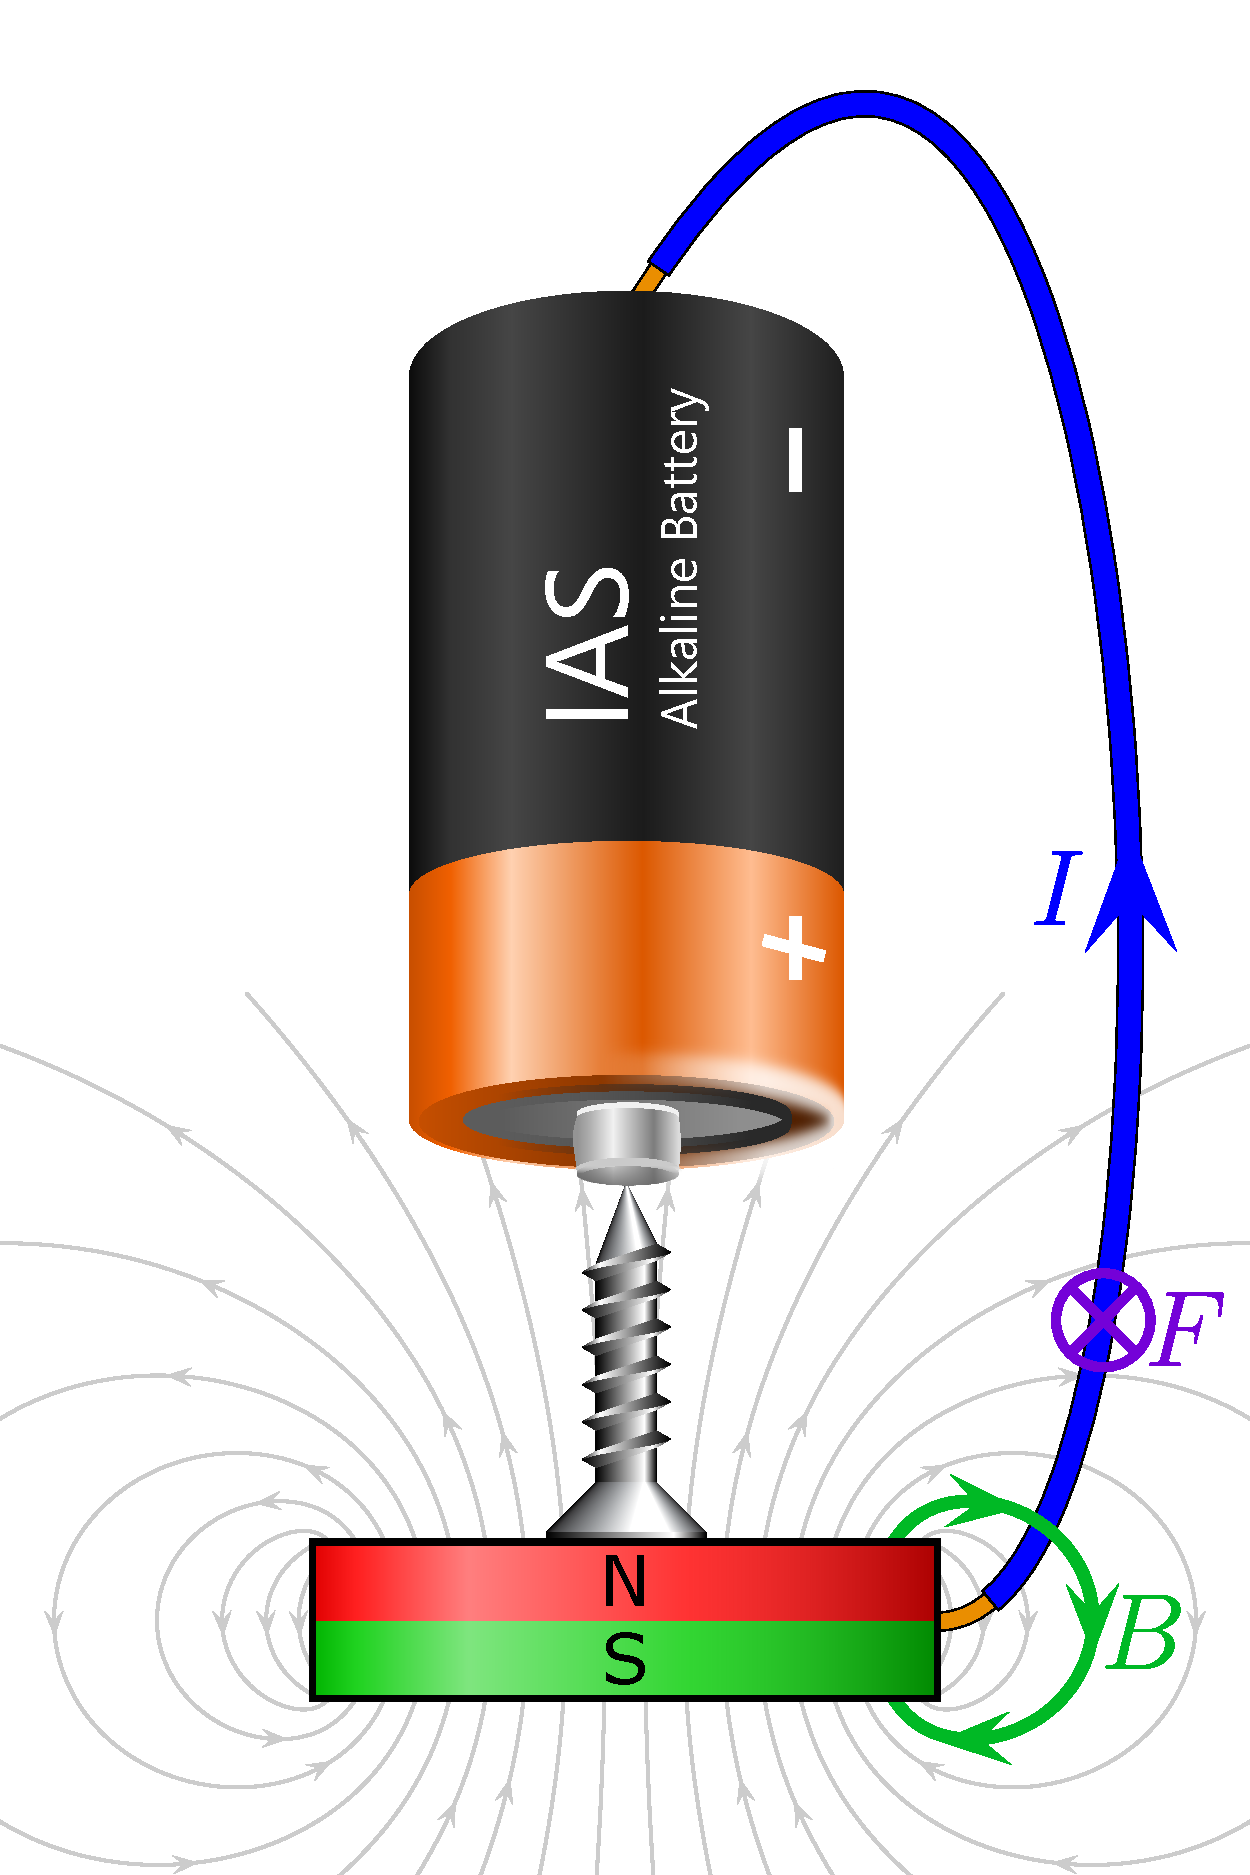
\includegraphics[width=0.47\textwidth]{fig/lec03/Homopolar_machine.pdf}
			\caption{Electric current, magnetic field and Lorentz force (adapted: \href{https://commons.wikimedia.org/wiki/File:Homopolar-motor.svg}{Wikimedia Commons}, M. Run, \href{https://creativecommons.org/licenses/by-sa/4.0/deed.en}{CC BY-SA})}
		\end{subfigure}
		\caption{Working principle of homopolar machines demonstrated with a simple permanent magnet, battery and screw design} 
        \label{fig:Homopolar_machine}
	\end{figure}
\end{frame}


%%%%%%%%%%%%%%%%%%%%%%%%%%%%%%%%%%%%%%%%%%%%%%%%%%%%%%%%%%%%%
%% Homopolar / unipolar machines (cont.) %%
%%%%%%%%%%%%%%%%%%%%%%%%%%%%%%%%%%%%%%%%%%%%%%%%%%%%%%%%%%%%%
\begin{frame}
	\frametitle{Homopolar / unipolar machines (cont.)}
    \begin{columns}
		\begin{column}{0.5\textwidth}
            \begin{itemize}
                \item  Homopolar machines are the simplest form of electric machines.
                \item They are also true DC machines, as the current and flux paths are unidirectional.
                \item The general design prevents connecting multiple rotor turns in series to increase the voltage, that is, only a relatively low voltage is induced.
                \item Consequently, homolpolar machines require high currents (in the order of  \si{\kilo\ampere} or even \si{\mega\ampere}) to reach a useful power range which limited their application.
            \end{itemize}
		\end{column}
        \hfill
		\begin{column}{0.49\textwidth}
			\begin{figure}
				\centering
				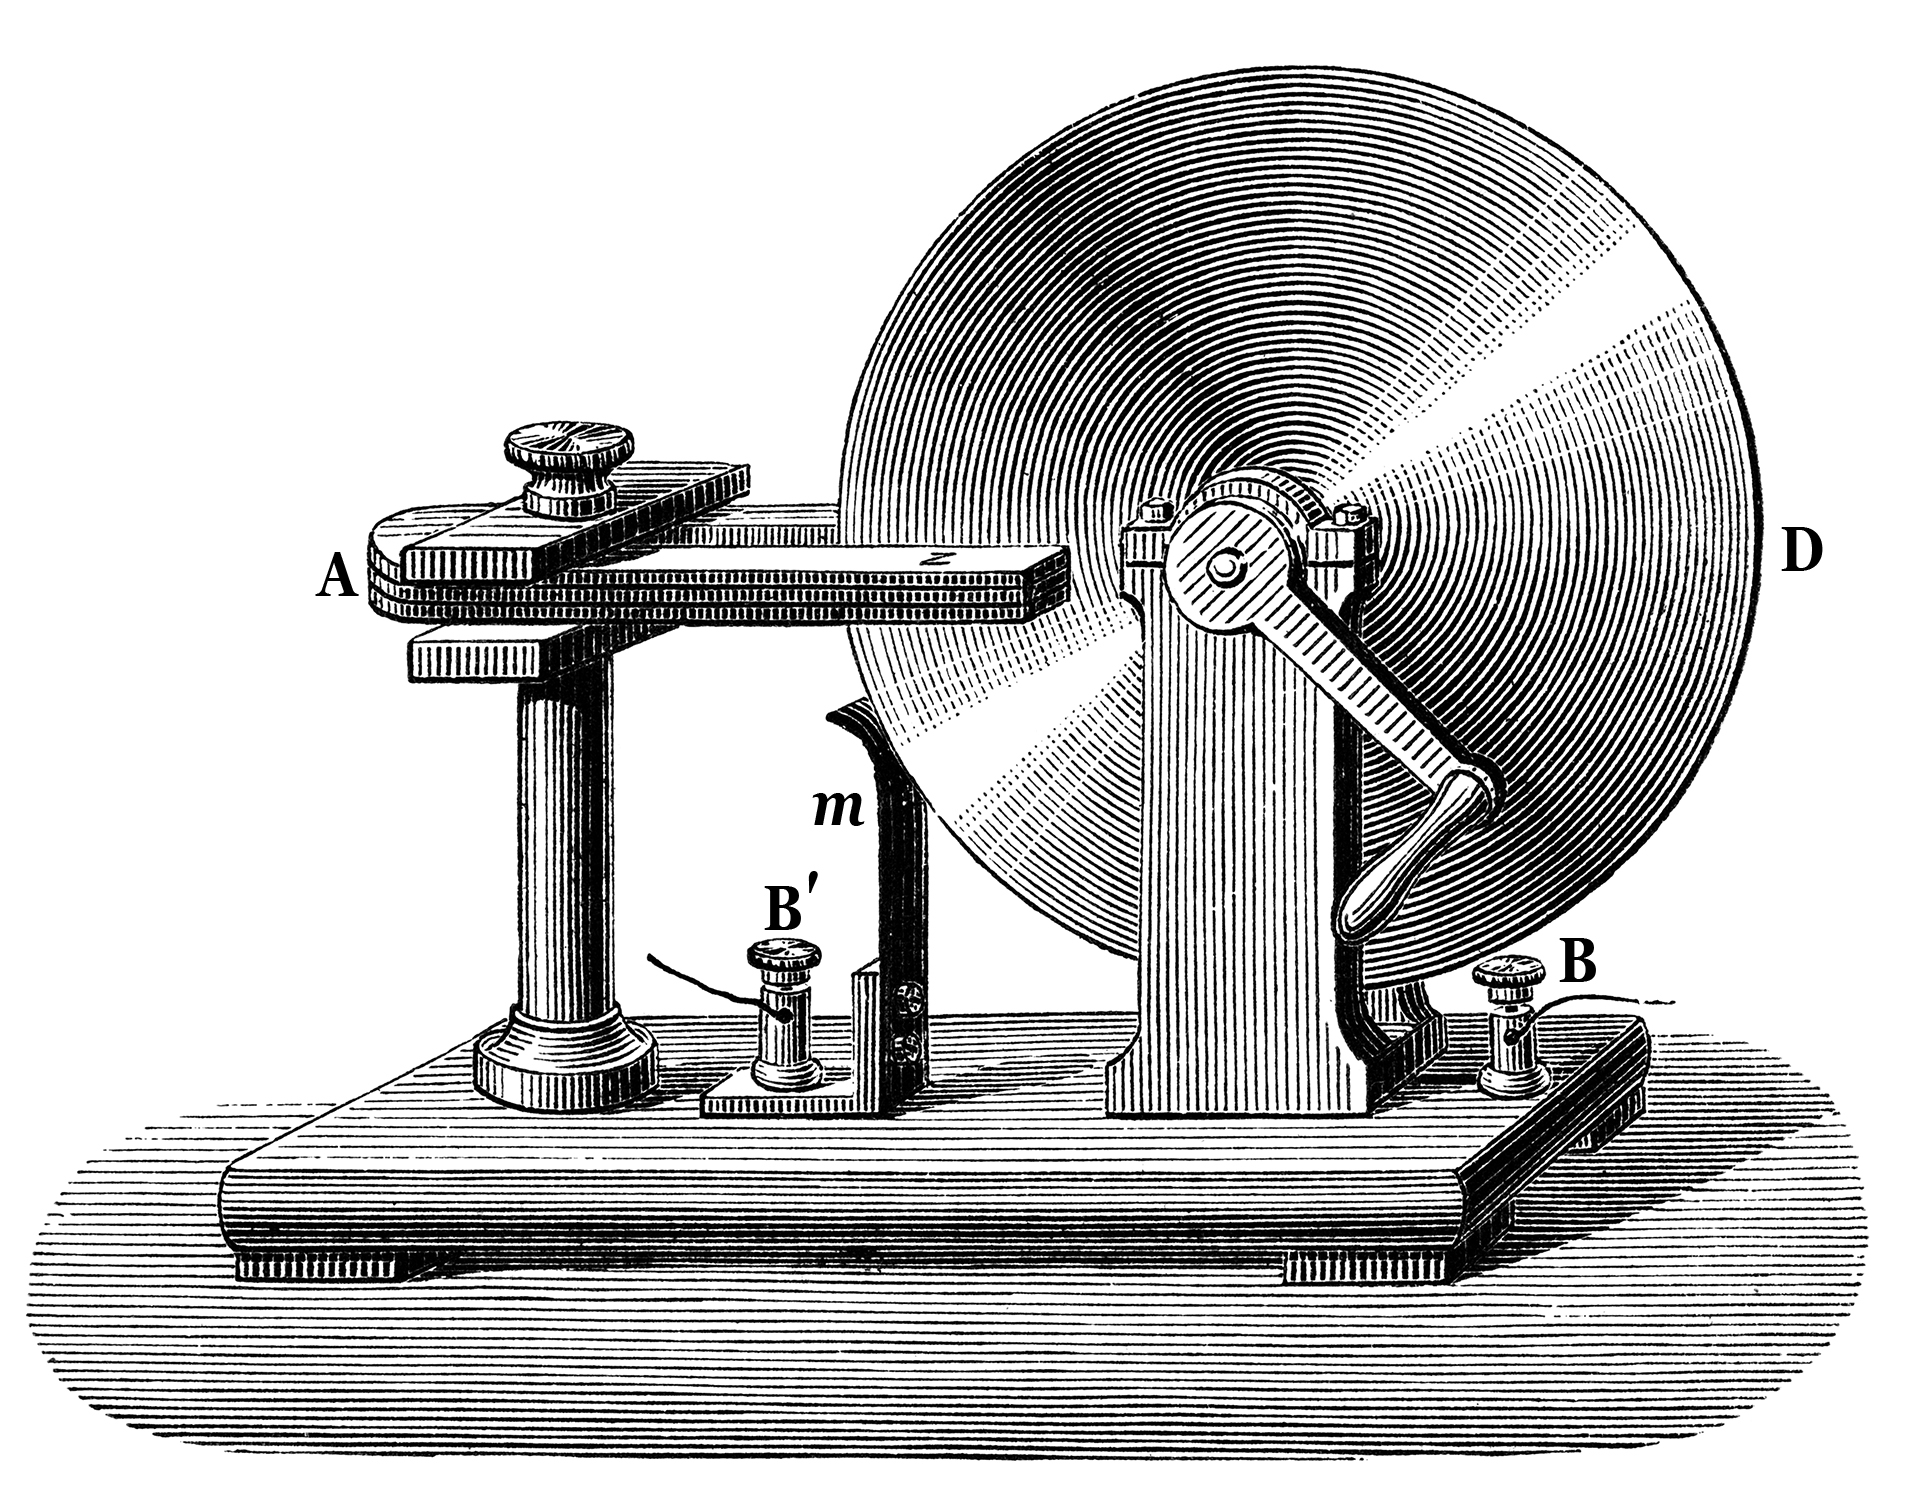
\includegraphics[width=0.8\textwidth]{fig/lec03/Faraday_disk_generator.jpg}
				\caption{The Faraday disk: another homopolar machine (source: \href{https://commons.wikimedia.org/wiki/File:Faraday_disk_generator.jpg}{Wikimedia Commons}, public domain)}
			\end{figure}
		\end{column}
		\end{columns}
\end{frame}

%%%%%%%%%%%%%%%%%%%%%%%%%%%%%%%%%%%%%%%%%%%%%%%%%%%%%%%%%%%%%
%% Working principle of usual DC machines %%
%%%%%%%%%%%%%%%%%%%%%%%%%%%%%%%%%%%%%%%%%%%%%%%%%%%%%%%%%%%%%
\begin{frame}
	\frametitle{Working principle of usual DC machines}
    \begin{columns}
		\begin{column}{0.5\textwidth}
            Let's consider \figref{fig:Simple_yoke_coil} and assume that the flux density $B$ is constant in the air gap and that the conductor loop has a length $l$. According to the Lorentz force we have
			\begin{equation}
				F = i_\mathrm{A} B l .
			\end{equation}  
			The torque $T$ on the conductor loop is given by
			\begin{equation}
				T = 2 F \frac{d}{2} \cos\left(\alpha\right) = i_\mathrm{A} B l d \cos\left(\alpha\right).
			\end{equation}
			If the loop spins with an angular velocity $\omega$, mechanical power $P_\mathrm{me} = T\omega$ is produced. 
			\\[1em]
			\textbf{Question:} What is happening if the coil is outside the magnetic field?
		\end{column}
        \hfill
		\begin{column}{0.49\textwidth}
			\begin{figure}
				\centering
				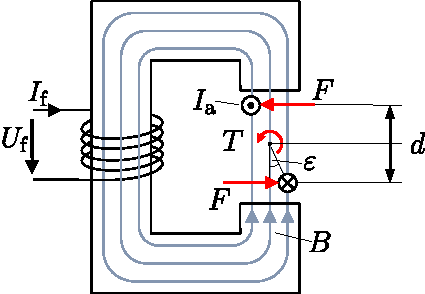
\includegraphics[width=0.9\textwidth]{fig/lec03/Simple_yoke_coil.pdf}
				\caption{Torque on a conductor loop (adapted from J.~B\"ocker, \textit{Elektrische Antriebstechnik}, Paderborn University, 2020)}
				\label{fig:Simple_yoke_coil}
			\end{figure}
		\end{column}
		\end{columns}
\end{frame}

%%%%%%%%%%%%%%%%%%%%%%%%%%%%%%%%%%%%%%%%%%%%%%%%%%%%%%%%%%%%%
%% DC-machine cross section %%
%%%%%%%%%%%%%%%%%%%%%%%%%%%%%%%%%%%%%%%%%%%%%%%%%%%%%%%%%%%%%
\begin{frame}
	\frametitle{DC-machine cross section}
    \begin{columns}
		\begin{column}{0.42\textwidth}
            \begin{itemize}
				\item To ensure a quasi-continous torque, the current through the conductor loop(s) in the rotor must have a constant direction.
				\item This is achieved by using a commutator (brushes).
				\item Compared to homopolar machines, DC machines require a mechanical rectification of the current.
			\end{itemize}
		\end{column}
        \hfill
		\begin{column}{0.55\textwidth}
			\begin{figure}
				\centering
				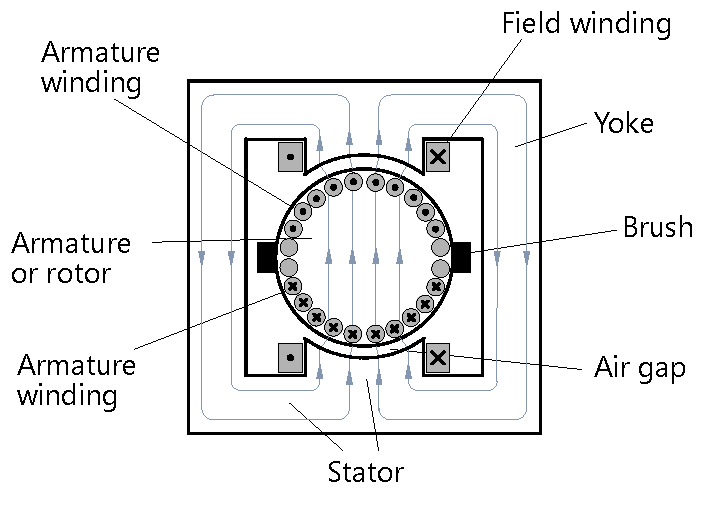
\includegraphics[width=0.925\textwidth]{fig/lec03/DC_machine_cross_section.pdf}
				\caption{Simplified DC machine cross section (adapted from J.~B\"ocker, \textit{Elektrische Antriebstechnik}, Paderborn University, 2020)}
				\label{fig:Simple_yoke_coil}
			\end{figure}
		\end{column}
		\end{columns}
\end{frame}

%%%%%%%%%%%%%%%%%%%%%%%%%%%%%%%%%%%%%%%%%%%%%%%%%%%%%%%%%%%%%
%% Commutation %%
%%%%%%%%%%%%%%%%%%%%%%%%%%%%%%%%%%%%%%%%%%%%%%%%%%%%%%%%%%%%%
\begin{frame}
	\frametitle{Commutation}
    \begin{figure}
		\centering
		\movie{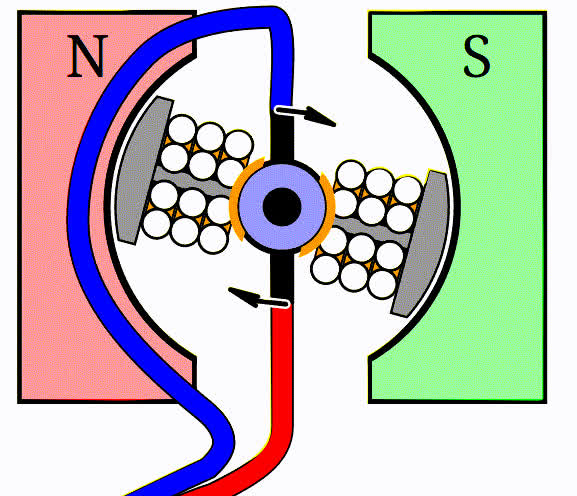
\includegraphics[height=0.65\textheight]{fig/lec03/DC_machine_simple_animation.jpeg}}{fig/lec03/DC_machine_simple_animation.gif}
		\caption{Animation of the commutation process \\(source: \href{https://commons.wikimedia.org/wiki/File:Animation_einer_Gleichstrommaschine_(Variante-Langsam).gif}{Wikimedia Commons}, M. Frey, \href{https://creativecommons.org/licenses/by-sa/3.0/deed.en}{CC BY-SA 3.0})}
	\end{figure}
\end{frame}

%%%%%%%%%%%%%%%%%%%%%%%%%%%%%%%%%%%%%%%%%%%%%%%%%%%%%%%%%%%%%
%% Armature and commutator %%
%%%%%%%%%%%%%%%%%%%%%%%%%%%%%%%%%%%%%%%%%%%%%%%%%%%%%%%%%%%%%
\begin{frame}
	\frametitle{Armature and commutator}
    \begin{figure}
		\centering
		\begin{subfigure}[b]{0.49\textwidth}
			\centering
			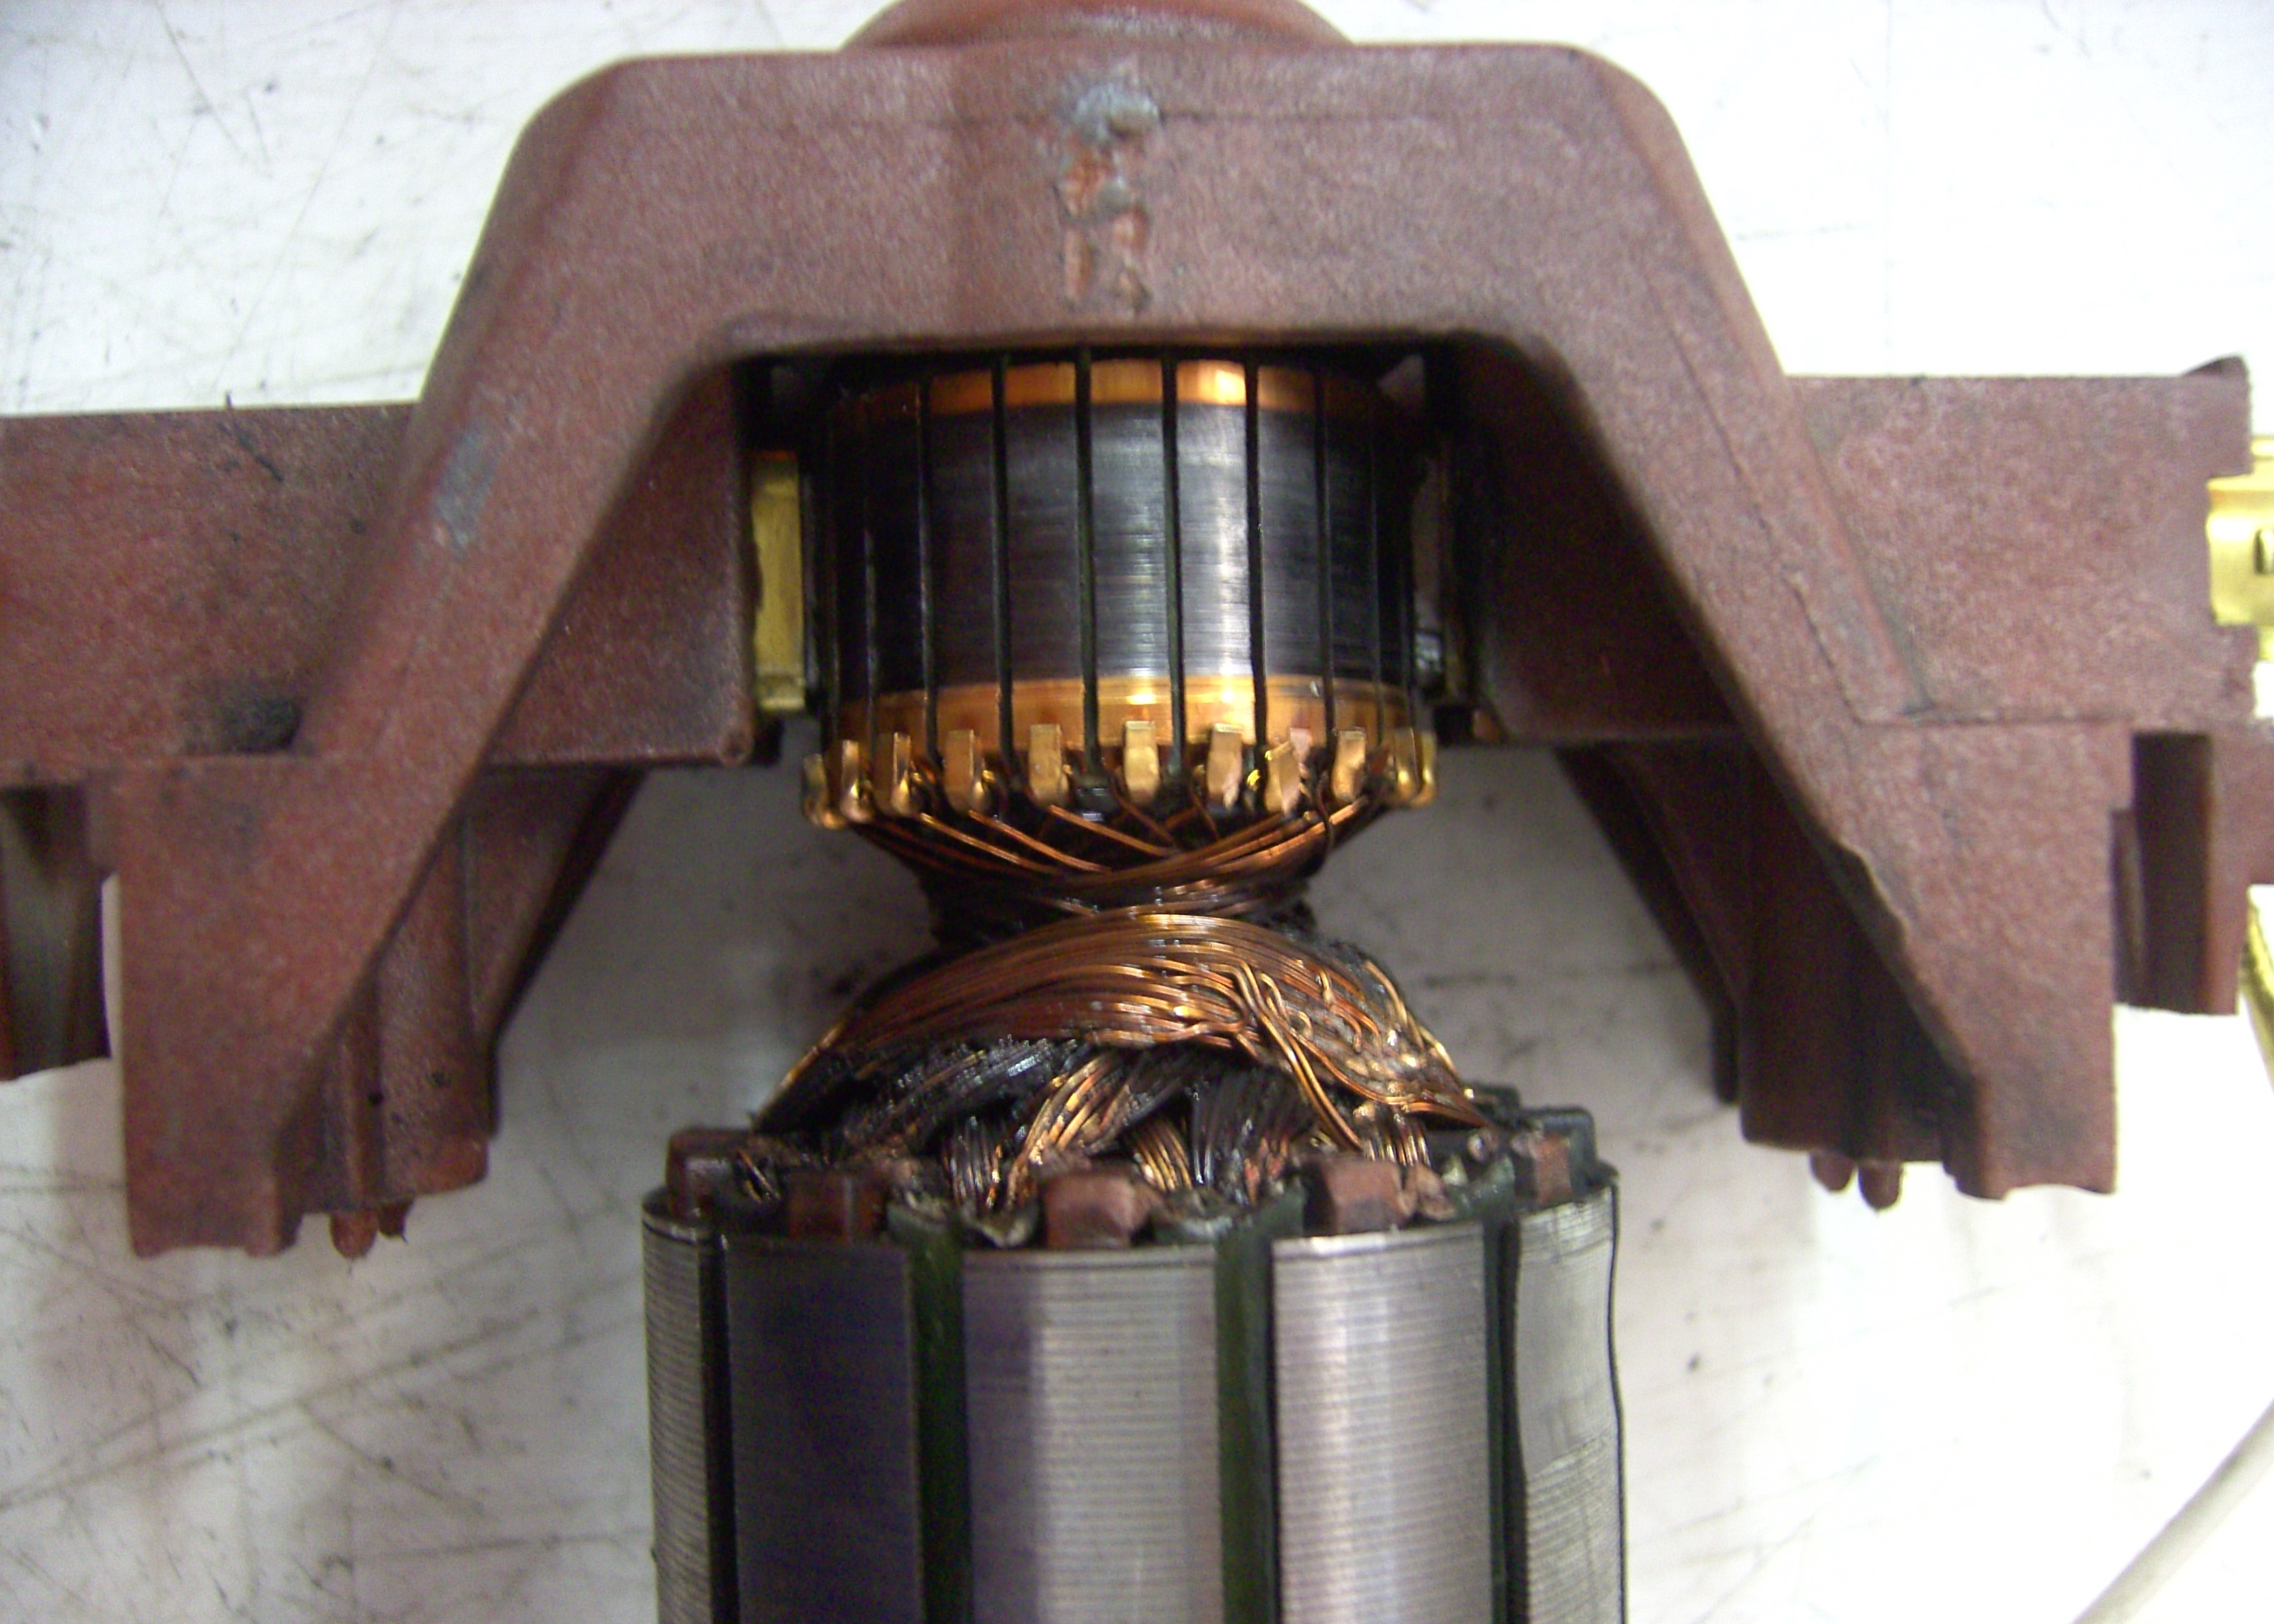
\includegraphics[width=0.85\textwidth]{fig/lec03/Commutator_Universalmachine.jpg}
			\caption{Commutator with brushes and springs (source: \href{https://commons.wikimedia.org/wiki/File:Kommutator_eines_Universalmotor.JPGg}{Wikimedia Commons}, Marrrci, \href{https://creativecommons.org/licenses/by-sa/3.0/deed.en}{CC BY-SA 3.0})}
		\end{subfigure}
		\hfill
		\begin{subfigure}[b]{0.49\textwidth}
			\centering
			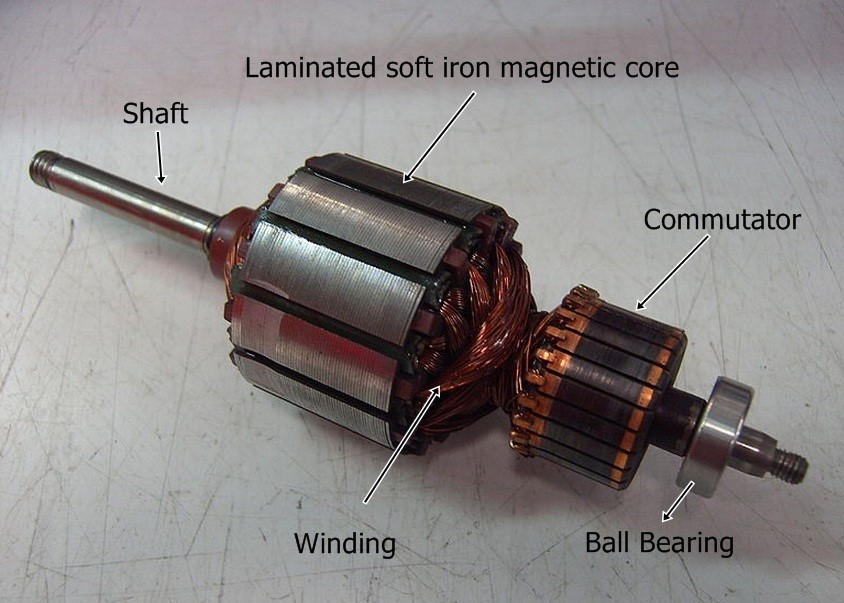
\includegraphics[width=0.85\textwidth]{fig/lec03/DC_armature_example.jpg}
			\caption{DC machine armature with commutator (source: \href{https://commons.wikimedia.org/wiki/File:Motor_rotor.jpg}{Wikimedia Commons}, public domain)}
		\end{subfigure}
		\caption{Examples of commutators and armatures} 
        \label{fig:Armature_and_commutator}
	\end{figure}
\end{frame}

%%%%%%%%%%%%%%%%%%%%%%%%%%%%%%%%%%%%%%%%%%%%%%%%%%%%%%%%%%%%%
%% Armature and commutator (cont.) %%
%%%%%%%%%%%%%%%%%%%%%%%%%%%%%%%%%%%%%%%%%%%%%%%%%%%%%%%%%%%%%
\begin{frame}
	\frametitle{Armature and commutator (cont.)}
    \begin{figure}
		\centering
		\begin{subfigure}[b]{0.49\textwidth}
			\centering
			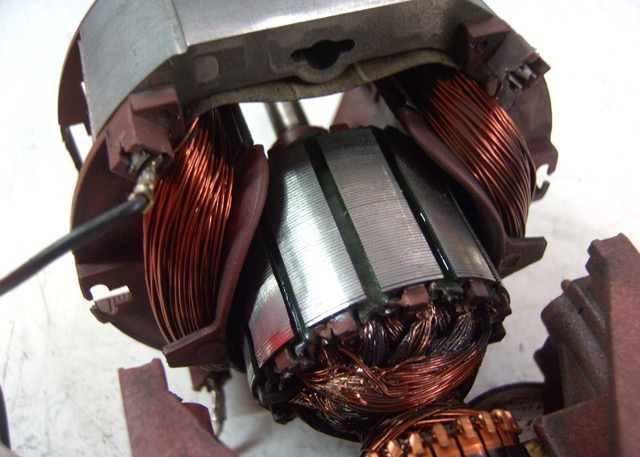
\includegraphics[width=0.85\textwidth]{fig/lec03/Stator_Rotor_Universalmachine.jpg}
			\caption{Armature inside stator (source: \href{https://commons.wikimedia.org/wiki/File:Universalmotor_1.JPG}{Wikimedia Commons}, Marrrci, \href{https://creativecommons.org/licenses/by-sa/3.0/deed.en}{CC BY-SA 3.0})}
		\end{subfigure}
		\hfill
		\begin{subfigure}[b]{0.49\textwidth}
			\centering
			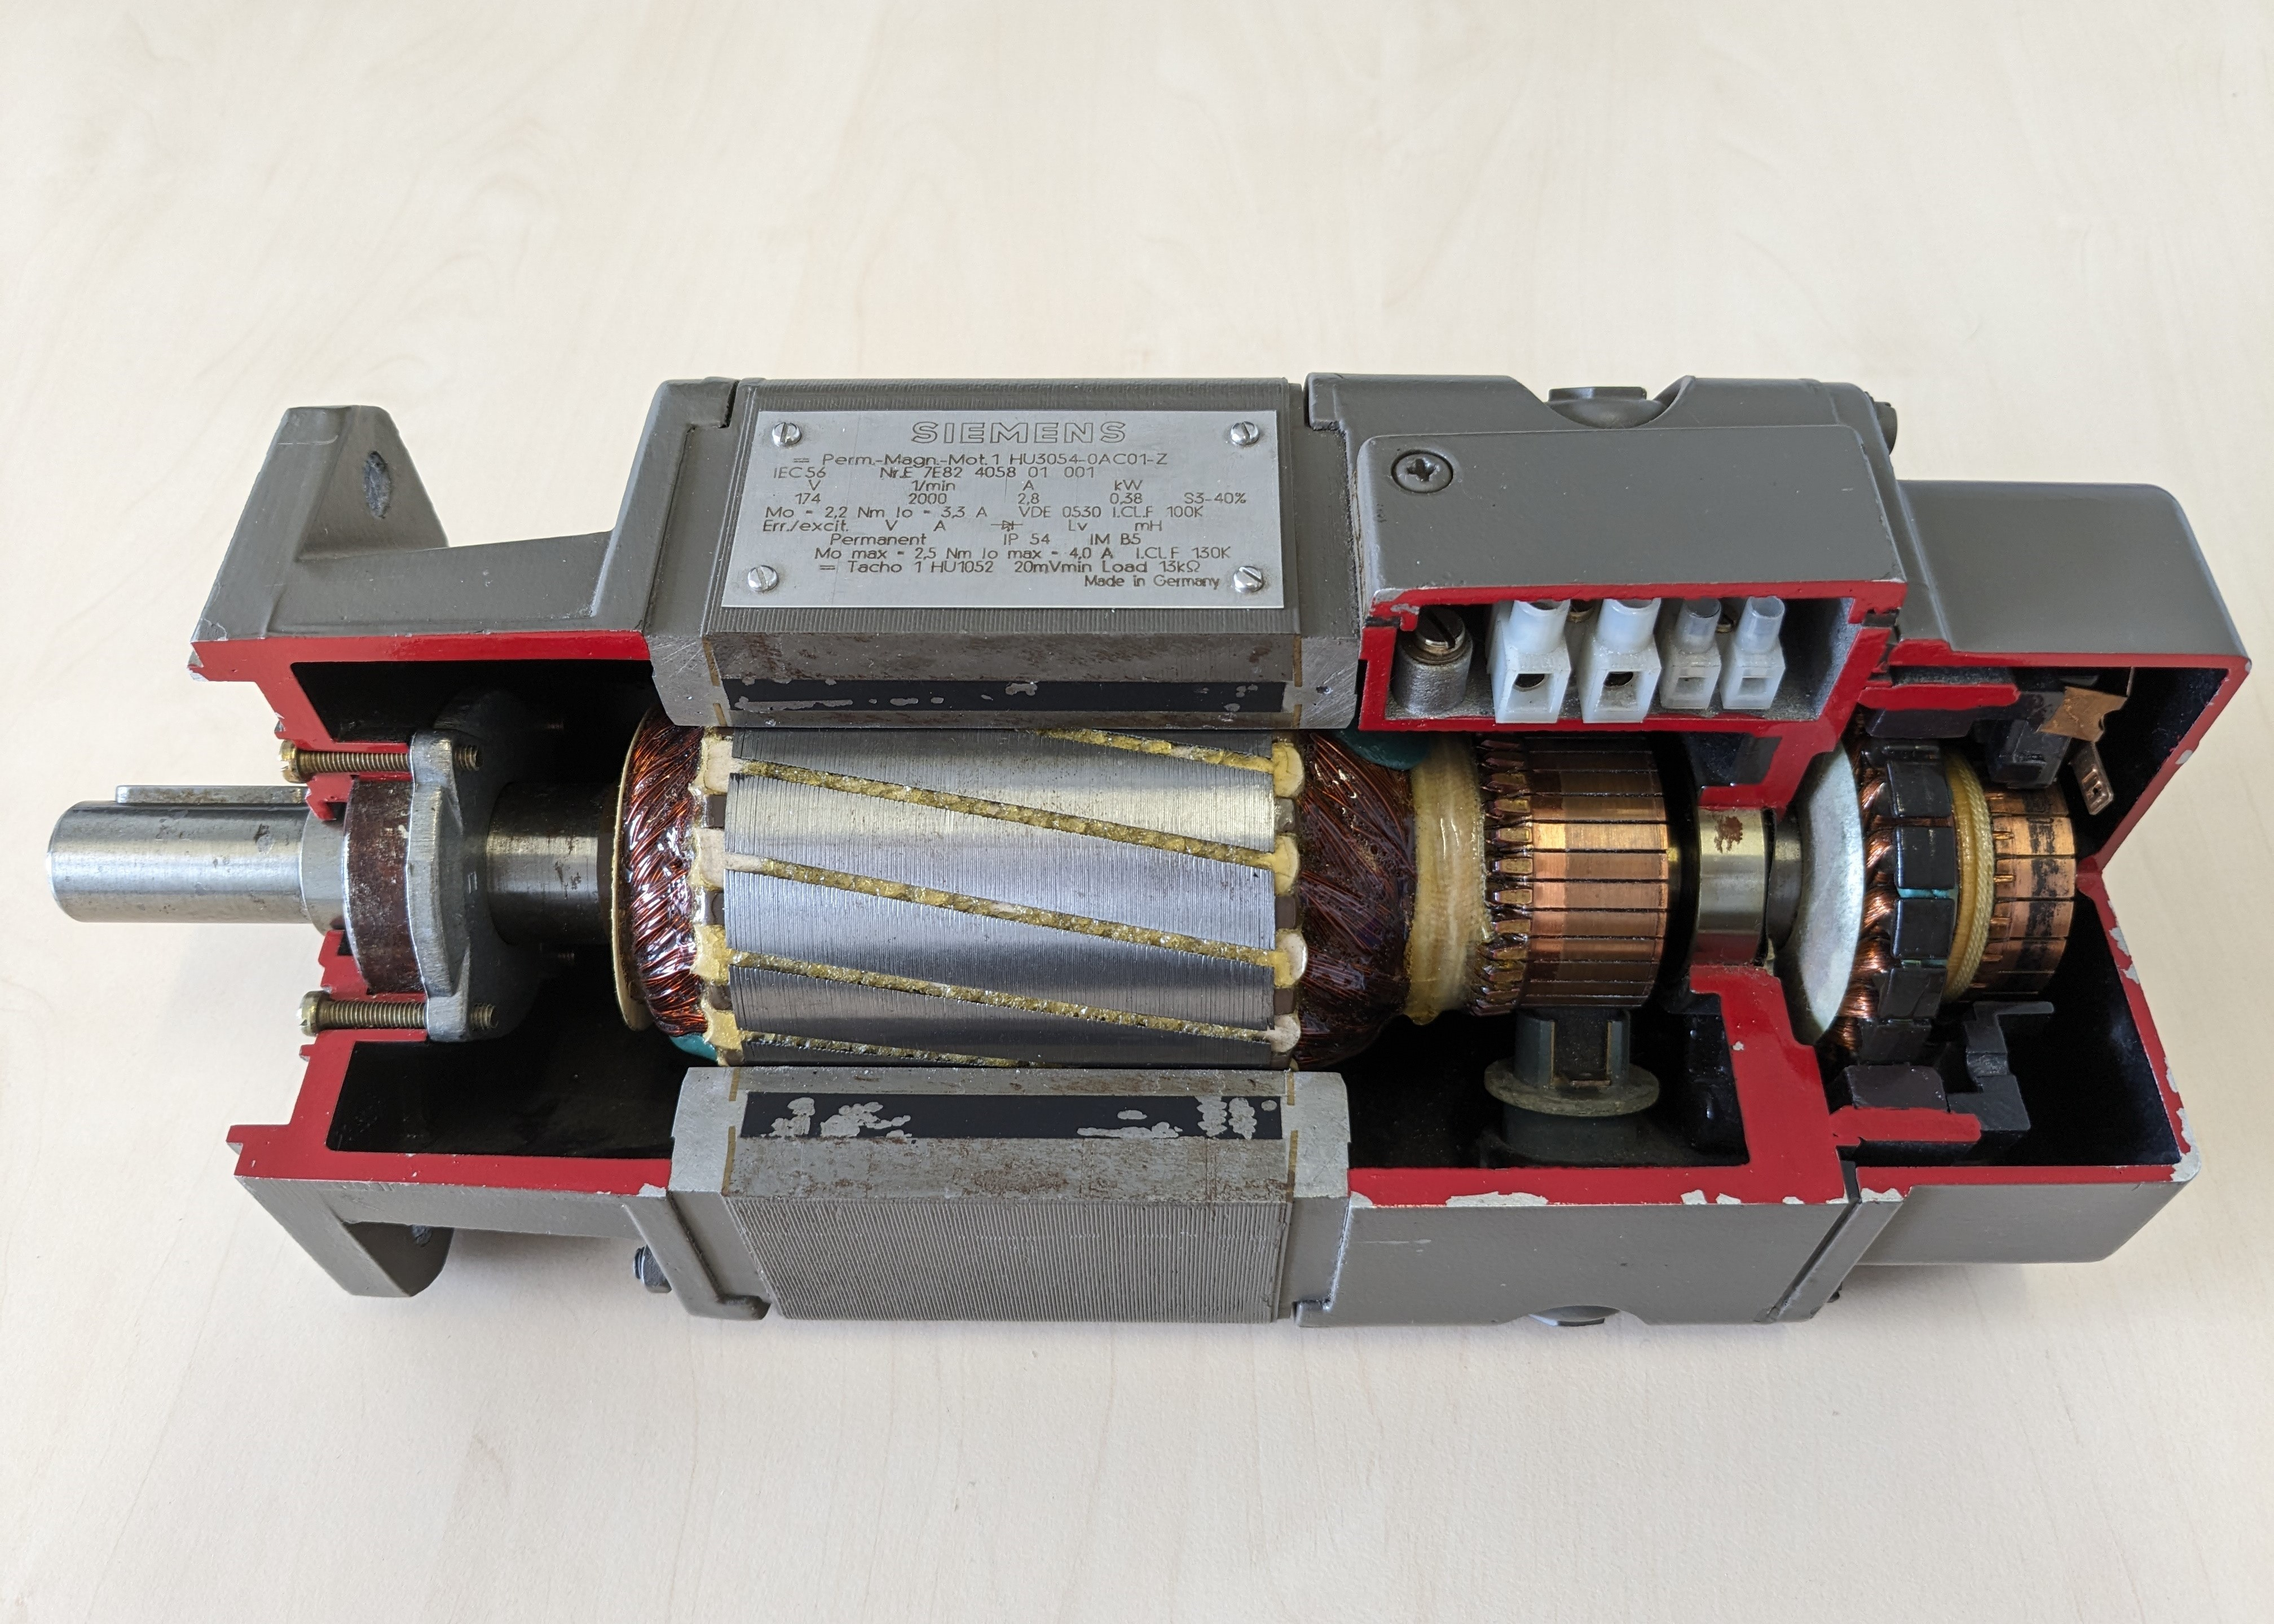
\includegraphics[width=0.85\textwidth]{fig/lec03/DC_Machine_PM.jpg}
			\caption{DC machine with permanent magnet excitation and tacho speed sensor}
		\end{subfigure}
		\caption{Examples of commutators and armatures (cont.)} 
        \label{fig:Armature_and_commutator_02}
	\end{figure}
\end{frame}

%%%%%%%%%%%%%%%%%%%%%%%%%%%%%%%%%%%%%%%%%%%%%%%%%%%%%%%%%%%%%
%% Commutation process with an armature lap winding %%
%%%%%%%%%%%%%%%%%%%%%%%%%%%%%%%%%%%%%%%%%%%%%%%%%%%%%%%%%%%%%
\begin{frame}
	\frametitle{Commutation process with an armature lap winding}
    \begin{figure}
        \centering
        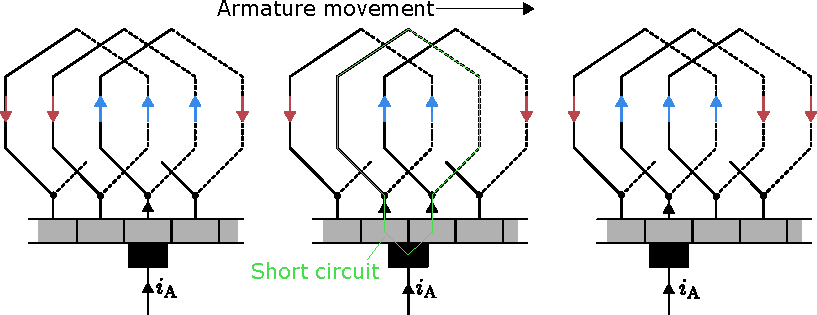
\includegraphics[height=0.6\textheight]{fig/lec03/Commutation_process_lap_winding.pdf}
        \caption{Three still images of the commutation process with a simplified winding representation (from left to right): when the brush touches two commutator segments, the according conductor loop is short-circuited and the current is reduced to zero. The brush then moves to the next commutator segment and the current starts flowing again but in a different direction.}
    \end{figure}
\end{frame}

%%%%%%%%%%%%%%%%%%%%%%%%%%%%%%%%%%%%%%%%%%%%%%%%%%%%%%%%%%%%%
%% Lap winding %%
%%%%%%%%%%%%%%%%%%%%%%%%%%%%%%%%%%%%%%%%%%%%%%%%%%%%%%%%%%%%%
\begin{frame}
	\frametitle{Lap winding}
    \begin{figure}
        \centering
        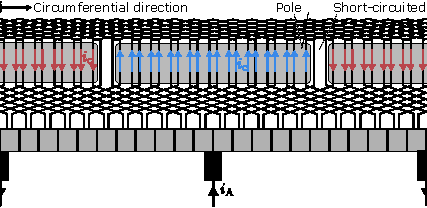
\includegraphics[height=0.65\textheight]{fig/lec03/Lap_winding.pdf}
        \caption{Lap winding with commutator unrolled along the circumferential coordinate}
    \end{figure}
\end{frame}